\chapter{The Drude and Drude--Sommerfeld Electron Gases}
\label{ch:drude-sommerfeld}

An electric field shifts the mean velocity of a collision-dominated thermal
gas.  Classical Maxwell--Boltzmann occupation gives the Drude model.
Fermi--Dirac occupation gives the Drude--Sommerfeld model and confines the
linear response of a degenerate gas to the Fermi window.

\section{The classical Drude response}

Taking the ensemble average of \cref{eq:thermal-gas-langevin} removes the
zero-mean stochastic term:
\begin{equation}
  m\frac{\dd\langle\bm V\rangle}{\dd t}
  =q_c\bm E-\frac{m}{\tau}\langle\bm V\rangle.
  \label{eq:drude-average-equation}
\end{equation}
After a constant field is applied at $t=0$,
\begin{equation}
  \langle\bm V(t)\rangle
  =\frac{q_c\tau}{m}\bm E
   \left(1-e^{-t/\tau}\right).
  \label{eq:drude-transient-velocity}
\end{equation}
The steady drift velocity is
\begin{equation}
  \bm v_{\mathrm d}=\frac{q_c\tau}{m}\bm E.
  \label{eq:drude-steady-velocity}
\end{equation}
For carrier density $n$, the charge-current density is
\begin{equation}
  \bm J=nq_c\bm v_{\mathrm d}
  =\frac{nq_c^2\tau}{m}\bm E.
  \label{eq:drude-current}
\end{equation}
The DC conductivity is therefore
\begin{equation}
  \boxed{\sigma_0=\frac{nq_c^2\tau}{m}.}
  \label{eq:drude-dc-conductivity}
\end{equation}
For electrons, $q_c=-q$.  Electron drift is opposite the field, while
conventional current is parallel to it.

For a harmonic field proportional to $e^{-\mathrm i\omega t}$,
\cref{eq:drude-average-equation} gives
\begin{equation}
  \boxed{
  \sigma(\omega)=\frac{\sigma_0}{1-\mathrm i\omega\tau}.
  }
  \label{eq:drude-ac-conductivity}
\end{equation}
The response is nearly resistive for $\omega\tau\ll1$.  At
$\omega\tau\gtrsim1$, carrier momentum cannot relax within one field cycle and
the current acquires a substantial phase lag.

The mechanical mobility magnitude is
\begin{equation}
  \mu=\frac{|q_c|\tau}{m}.
  \label{eq:drude-mobility}
\end{equation}
Combining this result with \cref{eq:thermal-gas-diffusivity} gives the Einstein
relation
\begin{equation}
  \boxed{D=\frac{\mu\kb T}{|q_c|}.}
  \label{eq:drude-einstein-relation}
\end{equation}
Diffusion and field-driven mobility contain the same momentum-relaxation time.

\begin{figure}[htbp]
  \centering
  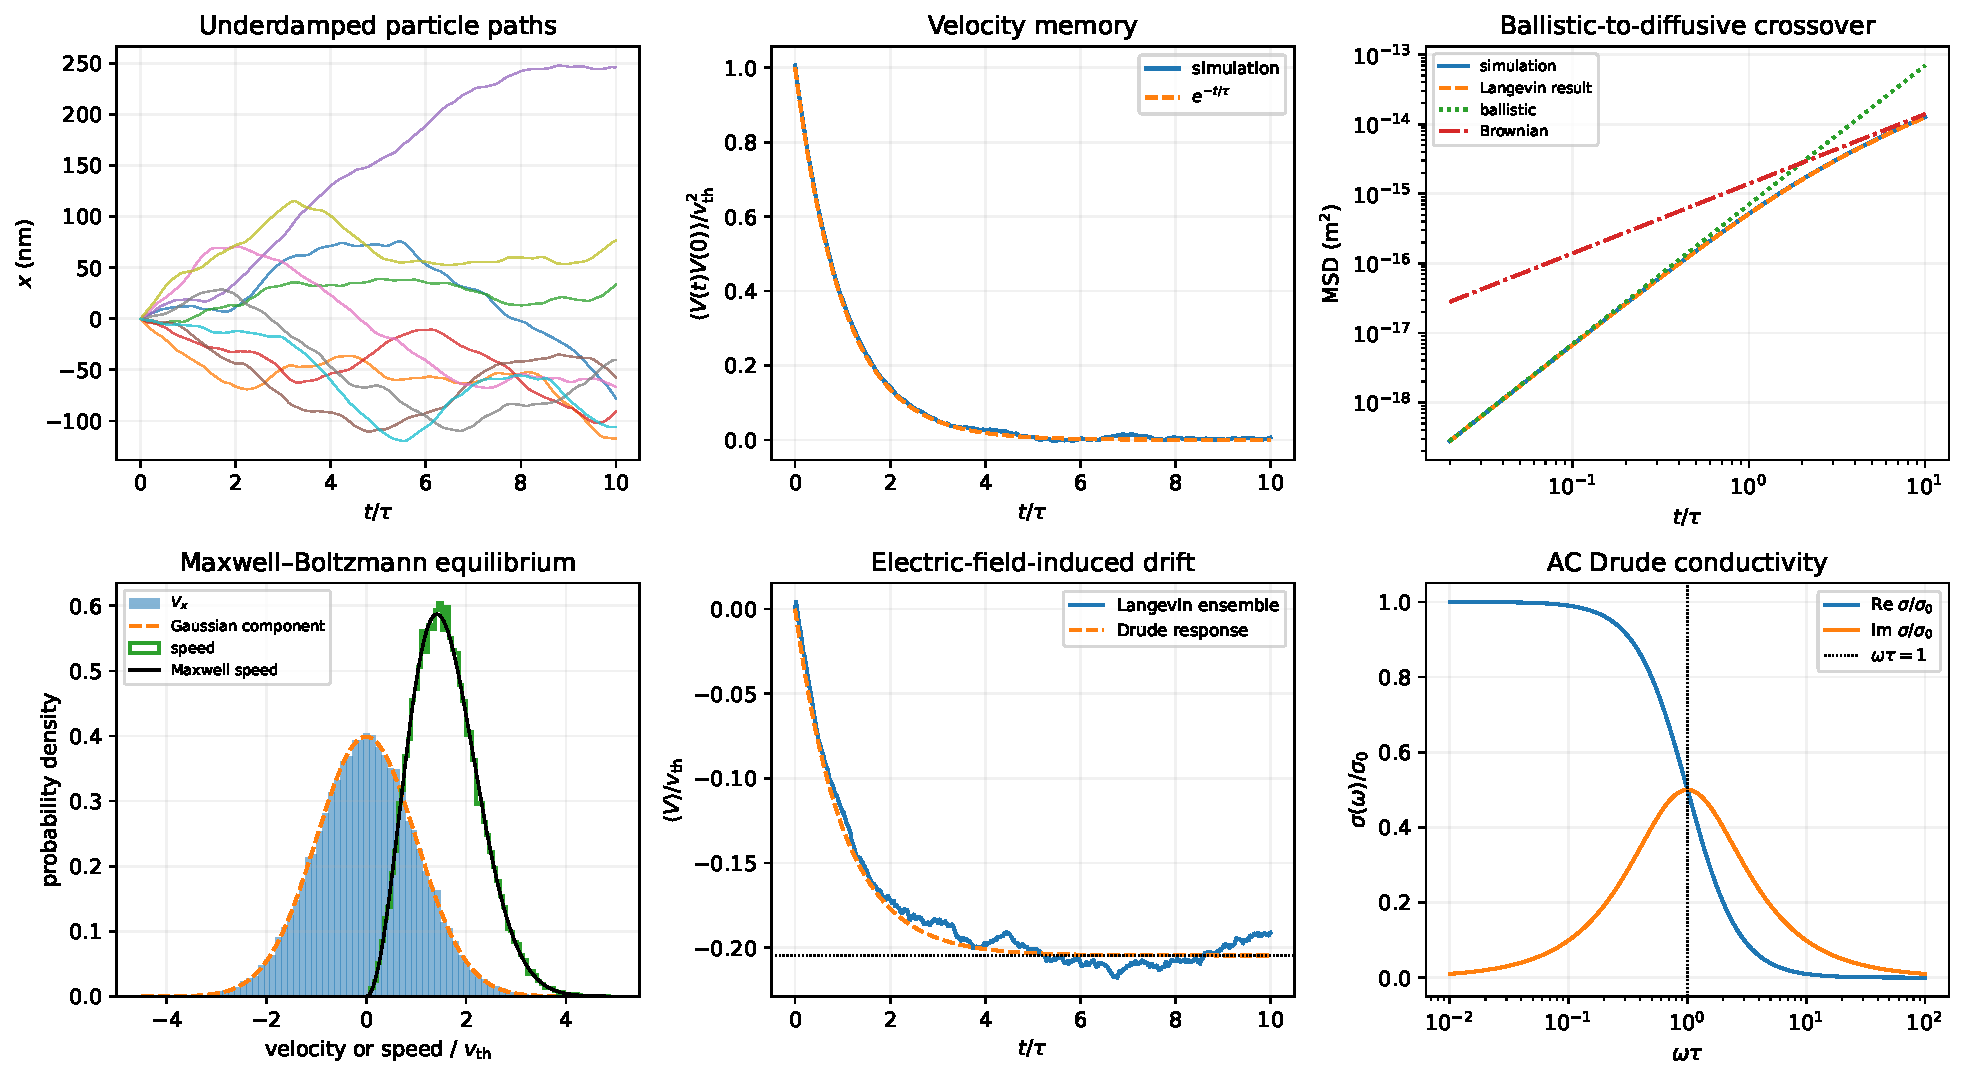
\includegraphics[width=\textwidth]
    {figures/08_brownian-motion-diffusion/lab-04-langevin-maxwell-boltzmann-drude.pdf}
  \caption{One Langevin model produces Maxwell--Boltzmann velocity statistics,
  the ballistic-to-diffusive crossover, field-induced Drude drift, and the
  frequency-dependent conductivity.\figurenotebookmark}
  \label{fig:thermal-gas-langevin-drude}
\end{figure}
\footnotetext{\textit{Student reproduction notebook:}
  \href{run:figures/08_brownian-motion-diffusion/lab-04-langevin-maxwell-boltzmann-drude.ipynb}
  {\texttt{Lab 4: Langevin, Maxwell--Boltzmann, and Drude transport}}.}

\section{The Sommerfeld correction}

The classical Drude model assigns Maxwell--Boltzmann statistics to the electron
gas.  Electrons are fermions.  Their equilibrium occupation is
\begin{equation}
  f_0(E)=\frac{1}{e^{(E-\mu)/(\kb T)}+1}.
  \label{eq:sommerfeld-fermi-distribution}
\end{equation}
For a band $E_n(\bm k)$, the semiclassical velocity is
\begin{equation}
  \bm v_n(\bm k)=\frac1\hbar\nabla_{\bm k}E_n(\bm k).
  \label{eq:sommerfeld-band-velocity}
\end{equation}
In the relaxation-time approximation, a weak uniform field changes the
occupation by
\begin{equation}
  \delta f_{n\bm k}
  =q_c\tau_{n\bm k}
   \bigl(\bm E\cdot\bm v_n(\bm k)\bigr)
   \left(-\frac{\partial f_0}{\partial E}\right).
  \label{eq:sommerfeld-linearized-distribution}
\end{equation}
The resulting conductivity tensor is
\begin{equation}
  \boxed{
  \sigma_{ij}
  =q_c^2g_s\sum_n
   \int_{\mathrm{BZ}}\frac{\dd^3k}{(2\pi)^3}
   \tau_{n\bm k}v_{n,i}v_{n,j}
   \left(-\frac{\partial f_0}{\partial E}\right).
  }
  \label{eq:sommerfeld-conductivity}
\end{equation}
The factor $-\partial f_0/\partial E$ is the Fermi window.  In a degenerate
gas, it restricts linear-response transport to states close to the chemical
potential.  The filled states far below the chemical potential do not produce
a net current because opposite velocities cancel.

For an isotropic parabolic band and constant $\tau$,
\cref{eq:sommerfeld-conductivity} reduces to the Drude form
$nq_c^2\tau/m$.  The Drude--Sommerfeld model retains the relaxation-time
equation of motion and replaces classical occupation by Fermi--Dirac
occupation.  This replacement corrects the electronic heat capacity and the
population of current-carrying states without treating the microscopic origin
of scattering.

\section{Range of validity}

The Drude model uses a parabolic free-electron dispersion, independent
collisions, and a phenomenological momentum-relaxation time.  The Sommerfeld
correction replaces classical occupation by Fermi--Dirac occupation but retains
the relaxation-time description.  Energy-dependent and anisotropic scattering,
strong fields, magnetic quantization, and coherent transport require a more
complete collision or quantum-transport model.

\section{Chapter summary}

A constant electric field produces the steady drift velocity
$\bm v_{\mathrm d}=q_c\tau\bm E/m$ and the Drude conductivity
$\sigma_0=nq_c^2\tau/m$.  A harmonic field gives
$\sigma(\omega)=\sigma_0/(1-\mathrm i\omega\tau)$.  Fermi--Dirac occupation
replaces the classical gas by the Drude--Sommerfeld gas.  Its conductivity is a
Fermi-window integral of velocity products and relaxation times.  The next
chapter replaces the vacuum dispersion by crystal-band velocity and effective
mass.
